%%%%%%%%%%%%%%%%%%%%%%%%%%%%%%%%%%%%%%%%%%%%%%%%%%%%%%%%%%%%%%%%%%%%%%%%%%%%%%%%
% Preamble
%%%%%%%%%%%%%%%%%%%%%%%%%%%%%%%%%%%%%%%%%%%%%%%%%%%%%%%%%%%%%%%%%%%%%%%%%%%%%%%%
\documentclass{pset}
\usepackage{2110}
\usepackage{graphicx}
\usepackage{float}
\usepackage{amsmath}
\usepackage{tabularx}
\usepackage{wrapfig}
\usepackage{tikz}
\usetikzlibrary{shapes,backgrounds}


\newcommand{\athree}{A3}
\newcommand{\afive}{A5}
\newcommand{\asix}{A6}
\newcommand{\dfs}{Depth First Search}
\newcommand{\abutt}{\java{AbstractButterfly}}
\newcommand{\butt}{\java{Butterfly}}
\newcommand{\cms}{the CMS}

\newcommand{\removed}{This feature has been removed.}

%%%%%%%%%%%%%%%%%%%%%%%%%%%%%%%%%%%%%%%%%%%%%%%%%%%%%%%%%%%%%%%%%%%%%%%%%%%%%%%%
% Document
%%%%%%%%%%%%%%%%%%%%%%%%%%%%%%%%%%%%%%%%%%%%%%%%%%%%%%%%%%%%%%%%%%%%%%%%%%%%%%%%
\begin{document}

%%%%%%%%%%%%%%%%%%%%%%%%%%%%%%%%%%%%%%%%%%%%%%%%%%%%%%%%%%%%%%%%%%%%%%%%%%%%%%%%
% Conditional Compilation
%%%%%%%%%%%%%%%%%%%%%%%%%%%%%%%%%%%%%%%%%%%%%%%%%%%%%%%%%%%%%%%%%%%%%%%%%%%%%%%%
\ifx \ATHREE \undefined \else
\newcommand{\TITLEPAGE}{} 
\newcommand{\TOC}{} 
\newcommand{\OVERVIEW}{} 
\newcommand{\COURSEOVERVIEW}{} 
\newcommand{\DANAUSOVERVIEW}{} 
\newcommand{\SIMULATIONBASICS}{} 
\newcommand{\PARKSMAPSTILES}{} 
\newcommand{\BUTTERFLIES}{} 
%\newcommand{\POWER}{} 
\newcommand{\DIRECTION}{} 
%\newcommand{\SPEED}{} 
%\newcommand{\TURNSTIMING}{} 
\newcommand{\MAPS}{} 
\newcommand{\TILETYPES}{} 
%\newcommand{\CONNECTIVITY}{}
\newcommand{\TILESTATE}{} 
%\newcommand{\RANDOMMAPCONSTRUCTION}{} 
\newcommand{\BUTTERFLYAPI}{} 
\newcommand{\VOIDFLY}{} 
%\newcommand{\VOIDFLYSAFE}{} 
%\newcommand{\VOIDLAND}{} 
%\newcommand{\BOOLEANCOLLECT}{} 
\newcommand{\VOIDREFRESHSTATE}{} 
%\newcommand{\POWERGETPOWER}{} 
\newcommand{\INTGETMAPWIDTH}{} 
\newcommand{\INTGETMAPHEIGHT}{} 
\newcommand{\LEARNINGRUNNING}{} 
\newcommand{\LEARNING}{} 
\newcommand{\RUNNING}{} 
\newcommand{\CLO}{} 
\newcommand{\ADVICE}{} 
\newcommand{\CREDITS}{}
\fi

\ifx \ASIX \undefined \else
\newcommand{\TITLEPAGE}{} 
\newcommand{\TOC}{} 
\newcommand{\OVERVIEW}{} 
\newcommand{\COURSEOVERVIEW}{} 
\newcommand{\DANAUSOVERVIEW}{} 
\newcommand{\SIMULATIONBASICS}{} 
\newcommand{\PARKSMAPSTILES}{} 
\newcommand{\BUTTERFLIES}{} 
\newcommand{\POWER}{} 
\newcommand{\DIRECTION}{} 
\newcommand{\SPEED}{} 
\newcommand{\TURNSTIMING}{} 
\newcommand{\MAPS}{} 
\newcommand{\TILETYPES}{} 
\newcommand{\CONNECTIVITY}{}
\newcommand{\TILESTATE}{} 
\newcommand{\RANDOMMAPCONSTRUCTION}{} 
\newcommand{\BUTTERFLYAPI}{} 
\newcommand{\VOIDFLY}{} 
\newcommand{\VOIDFLYSAFE}{} 
\newcommand{\VOIDLAND}{} 
\newcommand{\BOOLEANCOLLECT}{} 
\newcommand{\VOIDREFRESHSTATE}{} 
\newcommand{\POWERGETPOWER}{} 
\newcommand{\INTGETMAPWIDTH}{} 
\newcommand{\INTGETMAPHEIGHT}{} 
\newcommand{\LEARNINGRUNNING}{} 
\newcommand{\LEARNING}{} 
\newcommand{\RUNNING}{} 
\newcommand{\CLO}{} 
\newcommand{\ADVICE}{} 
\newcommand{\CREDITS}{}
\fi

%%%%%%%%%%%%%%%%%%%%%%%%%%%%%%%%%%%%%%%%%%%%%%%%%%%%%%%%%%%%%%%%%%%%%%%%%%%%%%%%
% TITLEPAGE
%%%%%%%%%%%%%%%%%%%%%%%%%%%%%%%%%%%%%%%%%%%%%%%%%%%%%%%%%%%%%%%%%%%%%%%%%%%%%%%%
\ifx \TITLEPAGE \undefined \else
\clearpage
\vspace*{\fill}
\begin{center}
    \huge\bfseries
    Danaus Manual
\end{center}

\begin{figure}[H]
    \centering
    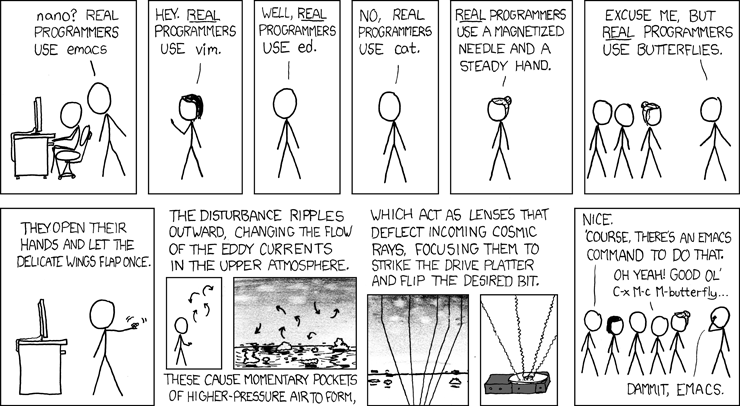
\includegraphics[width=\textwidth]{img/xkcd.png}
    \caption{Evidence you are all \emph{real} programmers.}
    \label{fig:xkcd}
\end{figure}
\vspace{\fill}
\clearpage
\fi

%%%%%%%%%%%%%%%%%%%%%%%%%%%%%%%%%%%%%%%%%%%%%%%%%%%%%%%%%%%%%%%%%%%%%%%%%%%%%%%%
% TOC
%%%%%%%%%%%%%%%%%%%%%%%%%%%%%%%%%%%%%%%%%%%%%%%%%%%%%%%%%%%%%%%%%%%%%%%%%%%%%%%%
\ifx \TOC \undefined \else
\newpage
\tableofcontents
\newpage
\fi

%%%%%%%%%%%%%%%%%%%%%%%%%%%%%%%%%%%%%%%%%%%%%%%%%%%%%%%%%%%%%%%%%%%%%%%%%%%%%%%%
% OVERVIEW
%%%%%%%%%%%%%%%%%%%%%%%%%%%%%%%%%%%%%%%%%%%%%%%%%%%%%%%%%%%%%%%%%%%%%%%%%%%%%%%%
\ifx \OVERVIEW \undefined \else
\section{Overview}
\ifx \COURSEOVERVIEW \undefined \else
\subsection{Course Overview}
Throughout the semester, you will be completing a large, multi-part
programming assignment in addition to several smaller, independent programming
assignments.

The multi-part programming series, known colloquially as Danaus\footnote{The
\link{http://en.wikipedia.org/wiki/Danaus_(genus)}{genus} of a butterfly.  Not
to be confused with the Greek god of the same name.}, will expose you to a
holistic, integrated form of object-oriented programming. For each assignment
in the three part series, you will be adding to the code you have previously
written to solve new challenges. Danaus will cover topics ranging from project
design and object orientation to graph exploration and traversal to machine
learning.

The smaller independent assignments will tax your skills with the fine-grained
details of object oriented programming.
\fi

\ifx \DANAUSOVERVIEW \undefined \else
\subsection{Danaus Overview}
In a nutshell, Danaus is a butterfly flight simulation engine. We have provided
a framework to generate pseudo-random maps, animate butterflies, and assess
their performance. You will be designing and programming the logic behind the
butterfly.

More specifically, yet with many details still elided, a simulation consists
mainly of a map, a butterfly, and some information on the state of the
simulation. A map is a toroidal grid of tiles. Each tile has a set of
attributes: light, wind, etc. A butterfly is placed within a map and can
explore the map by flying and landing. The goal of the butterfly is to collect
a set of flowers, distributed randomly throughout the map, as quickly and as
efficiently as possible. Throughout the simulation, various performance metrics
are recorded, such as total turns and time taken.

This document elaborates on the basics of a simulation, the attributes of a
map, the functionality of the butterfly API, etc. It is imperative that you
read and understand this document in full before you begin to design and
implement your butterfly.
\fi
\fi

%%%%%%%%%%%%%%%%%%%%%%%%%%%%%%%%%%%%%%%%%%%%%%%%%%%%%%%%%%%%%%%%%%%%%%%%%%%%%%%%
% Simulation Basics
%%%%%%%%%%%%%%%%%%%%%%%%%%%%%%%%%%%%%%%%%%%%%%%%%%%%%%%%%%%%%%%%%%%%%%%%%%%%%%%%
\ifx \SIMULATIONBASICS \undefined \else
\section{Simulation Basics}
This section provides an overview of Danaus' basics to help you form a
big-picture understanding of Danaus. The basics discussed here are explained in
greater detail in later sections. 
\ifx \PARKSMAPSTILES \undefined \else
\subsection{Parks, Maps, and Tiles}
Three important classes within Danaus are \java{Tile}, \java{Map}, and
\java{Park}.
\begin{itemize}
    \item \java{Tile}s, such as \java{Land} and \java{Water}, are the basic
      building blocks of Danaus. Butterflies travel to and from \java{Tile}s;
      \java{Aroma} and \java{Wind} are spread about \java{Tile}s; etc.
    \item A \java{Map} consists of an array of \java{Tile}s and some other
      bookkeeping information. A \java{Butterfly} interfaces most heavily with
      a \java{Map}. 
    \item A \java{Park} consists of a \java{Map} and some information about the
      state of a simulation. Butterflies do not directly interface with a
      \java{Park}, but a \java{Park} will record simulation statistics and
      performance metrics of the \java{Butterfly}.  
\end{itemize}

The hierarchical nature of \java{Tile}s, \java{Map}s, and \java{Park}s is
illustrated in Figure~\ref{fig:tileparkmap}.

\begin{figure}[h]
  \centering
  
  \def\firstcircle{(0,0) circle (1cm)}
  \def\secondcircle{(0,0) circle (2cm)}
  \def\thirdcircle{(0,0) circle (3cm)}

  \begin{tikzpicture}
    \begin{scope}[fill opacity=0.8]
        \fill[blue] \thirdcircle;
        \fill[green] \secondcircle;
        \fill[red] \firstcircle;
        \draw \firstcircle node[] {\java{Tile}};
        \draw \secondcircle node [above=1cm] {\java{Map}};
        \draw \thirdcircle node [above=2cm] {\java{Park}};
    \end{scope}
  \end{tikzpicture}
  \caption{The hierarchy of Danaus structures.}
  \label{fig:tileparkmap}
\end{figure}
\fi

\ifx \BUTTERFLIES \undefined \else
\subsection{Butterflies}
During a simulation, a butterfly both learns and runs on a map. When learning,
a butterfly exhaustively searches a map, collecting as much information about
the map as possible. When running, a butterfly collects a set of flowers in as
few turns as possible.
\fi

\ifx \POWER \undefined \else
\subsection{Power}
\removed{}
\fi

\ifx \DIRECTION \undefined \else
\subsection{Direction}
Directions, of enum \java{Direction}, are the eight basic cardinal directions:
N, NE, E, SE, S, SW, W, and NW\@. Each direction corresponds to one of a tile's
eight neighbors, as shown in Table~\ref{table:directions}.

\begin{table}[H]
  \centering
  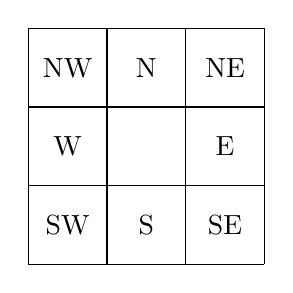
\begin{tikzpicture}
    \draw (0,0) grid (3,3);
    \node at (0.5,2.5) {NW};
    \node at (1.5,2.5) {N};
    \node at (2.5,2.5) {NE};
    \node at (2.5,1.5) {E};
    \node at (2.5,0.5) {SE};
    \node at (1.5,0.5) {S};
    \node at (0.5,0.5) {SW};
    \node at (0.5,1.5) {W};
  \end{tikzpicture}
  \caption{The relationship between cardinal directions and tile neighbors.}
  \label{table:directions}
\end{table}
\fi

\ifx \SPEED \undefined \else
\subsection{Speed}
\removed{}
\fi

% Much like real butterflies, Danaus butterflies can operate at different speeds.
% Danaus provides three speeds, which are defined in \java{enum Speed}:
% \java{SLOW}, \java{NORMAL}, and \java{FAST}. The speed affects the duration of
% a simulation. 
% \fi

\ifx \TURNSTIMING \undefined \else 
% \subsection{Turns and Timing}\label{sec:metrics}
% Danaus' simulation engine records various performance metrics during a
% butterfly's flight. Two related and important metrics are turns and time.
% 
% \subsubsection{Turns}
% \paragraph{turn}
% A park maintains an instance of \java{ParkState}, which represents the current
% state of the park. At the start of a simulation, field \java{ParkState.turn} is
% set to 0. \java{turn} is incremented every time a butterfly calls method
% \java{fly}, \java{flysafe}, or \java{land}. Even if a flying operation
% fails\footnote{A flying operation can fail if a butterfly flies into an
% obstacle or runs out of power mid-flight.}, the action is considered a turn
% and \java{turn} is incremented. \java{turn} can be thought of as the total
% number of steps that have passed in the simulation. 
% 
% \paragraph{slowSteps}
% Some actions in a simulation are slower than others. The speed of an action is
% reflected by \java{slowSteps}. Slower operations increment field
% \java{slowSteps}, average-paced operations do not affect \java{slowSteps},
% faster operations decrement \java{slowSteps}. You can think of \java{slowSteps}
% as a measure of your butterfly's speed.  Four actions  affect \java{slowSteps}.
% \begin{enumerate}
%     \item \textbf{Flying \java{SLOW}}. Flying slowly increments
%         \java{slowSteps}.
%     \item \textbf{Flying \java{NORMAL}}. Flying normally does not change
%         \java{slowSteps}.
%     \item \textbf{Flying \java{FAST}}. Flying quickly decrements
%         \java{slowSteps}.
%     \item \textbf{Flying over \java{Forest}}. Flying over forests decrements
%         \java{slowSteps}.
% \end{enumerate}
% 
% Non-mutually exclusive actions may both affect \java{slowSteps}. For example,
% flying slowly over \java{Forest}s decrements \java{slowSteps} by 2. Refer to
% Table~\ref{table:turns} for an example of how different operations affect
% turns.
% 
% \begin{table}[H]
%     \centering
%     \begin{tabular}{|l|c|c|c|c|}
%         \hline
%         \textbf{Operation} & \textbf{Speed} &  \textbf{Tile Type} &
%         \textbf{turn} & \textbf{slowSteps} \\\hline
%                       &        &        & 0 & 0 \\\hline
%         fly & Normal & Land   & 1 & 0 \\\hline 
%         fly & Normal & Land   & 2 & 0 \\\hline 
%         fly & Normal & Land   & 3 & 0 \\\hline 
%         fly & Slow   & Land   & 4 & 1 \\\hline 
%         fly & Slow   & Land   & 5 & 2 \\\hline 
%         fly & Slow   & Land   & 6 & 3 \\\hline 
%         fly & Fast   & Land   & 7 & 2 \\\hline 
%         fly & Fast   & Land   & 8 & 1 \\\hline
%         fly & Fast   & Forest & 9 & 1 \\\hline  
%         fly & Normal & Forest & 10 & 2 \\\hline  
%         fly & Slow   & Forest & 11 & 4 \\\hline  
%     \end{tabular}
%     \caption{Sample butterfly simulation with \java{turn} and \java{slowSteps}
%         listed. The listed turn is the state \textit{after} the operation has
%     completed.} \label{table:turns}
% \end{table}
% 
% \subsubsection{Timing}
% Turns reflect the concept of speed in the context of a simulation\footnote{e.g.
% flying slowly is twice as slow as flying at a normal pace.}. Timing reflects
% the actual runtime  of the program controlling a butterfly's logic. The faster
% and more efficient the algorithms, the less time is required to complete a
% simulation.
% 
% During a simulation, six times are recorded. The first three are the actual
% time of method \java{learn()}, the actual time of \java{run()}, and their
% sum\footnote{\java{learn} and \java{run} are described in detail in
% Section~\ref{sec:learnrun}.}. Actual time is, as its name implies, the actual
% duration of execution of a method call. The clock starts when a method is
% called and ends when the method terminates. The actual time does not include
% the time required by the framework to generate maps, render the GUI, etc. Only
% the performance of a butterfly's flight is timed. 
% 
% The last three measured times are adjusted times of \java{learn},  \java{run},
% and their sum. Similar to \java{slowSteps}, this time increases if a butterfly
% performs slower\footnote{Here, slower is used to reflect speed in the context
% of a simulation, not actual runtime speed.} operations. The adjusted time is
% calculated as follows. 
% \begin{gather*}
%     \text{tpm} = \frac{\text{time}_{\text{actual}}}{\text{turns}} \\
%     \text{time}_{\text{adjusted}} = \text{tpm} \times (\text{turns} +
%     \text{slowSteps})
% \end{gather*}
% where tpm is the actual time taken per turn. Note that if \java{slowSteps} is
% zero, then adjusted time equals actual time. If \java{slowSteps} is positive,
% adjusted time > actual time. If \java{slowSteps} is negative, adjusted time <
% actual time.
% 
% Table~\ref{table:metrics} explains the implications behind small values of
% \java{turn}, \java{slowSteps}, actual time, and adjusted time.
% 
% \begin{table}[H]
%     \center
%     \begin{tabularx}{\textwidth}{|l|X|}
%         \hline
%         \textbf{Metric} & \textbf{Small Metric Implies\ldots} \\\hline
%         turn &
%         The butterfly does not make unnecessary actions. It is efficient at
%         performing only the actions required to complete the
%         simulation.\\\hline
%         slowSteps &
%         The butterfly does not make unnecessary actions. It performs actions
%         that are relatively fast in the context of the simulation. \\\hline
%         actual time &
%         The time complexity of your algorithms is great. You do not perform
%         superfluous computations. You make every instruction count. \\\hline
%         adjusted time &
%         Not only are your algorithms fast but your butterfly is likely fast as
%         well. \\\hline
%     \end{tabularx}
%     \caption{Performance metrics.}
%     \label{table:metrics}
% \end{table}
% \fi
\fi


%%%%%%%%%%%%%%%%%%%%%%%%%%%%%%%%%%%%%%%%%%%%%%%%%%%%%%%%%%%%%%%%%%%%%%%%%%%%%%%%
% MAPS
%%%%%%%%%%%%%%%%%%%%%%%%%%%%%%%%%%%%%%%%%%%%%%%%%%%%%%%%%%%%%%%%%%%%%%%%%%%%%%%%
\ifx \MAPS \undefined \else
\section{Maps}\label{sec:maps}
\ifx \TILETYPES \undefined \else
\subsection{Tile Types}
A map is a toroidal grid of \java{Tile}s, each of which can be one of four
subclasses.
\subsubsection{Land}
\begin{wrapfigure}{l}{0.075\textwidth}
    \centering
    \vspace{-20pt}
    
\includegraphics{img/land.png}
    \vspace{-20pt}
\end{wrapfigure}
\java{Land}, the most basic type of \java{Tile}, is flat and flyable.

\subsubsection{Forest}
\begin{wrapfigure}{l}{0.075\textwidth}
    \centering
    \vspace{-20pt}
    
\includegraphics{img/forest_land.png}
    \vspace{-20pt}
\end{wrapfigure}
The tall and dense trees of a \java{Forest} tile are flyable.

\subsubsection{Cliff}
\begin{wrapfigure}{l}{0.075\textwidth}
    \centering
    \vspace{-20pt}
    
\includegraphics{img/cliff_land.png}
    \vspace{-20pt}
\end{wrapfigure}
A \java{Cliff} is towering and unflyable. When a butterfly tries to fly over a
\java{Cliff}, a \java{CliffCollisionException} is thrown, and the butterfly's
location does not change.

\subsubsection{Water}
\begin{wrapfigure}{l}{0.075\textwidth}
    \centering
    \vspace{-20pt}
    
\includegraphics{img/water.png}
    \vspace{-20pt}
\end{wrapfigure}
\java{Water} is treacherous and unflyable. When a butterfly tries to fly over
\java{Water}, a \java{WaterCollisionException} is thrown, and the butterfly's
location does not change.
\fi

\ifx \CONNECTIVITY \undefined \else
\subsection{Connectivity}
All maps are guaranteed to be connected. That is, there exists a path between
all pairs of flyable tiles. This implies that it is always possible for a
butterfly to explore every flyable tile in a map.
\fi

\ifx \TILESTATE \undefined \else
\subsection{Tile State}
Each tile also has a unique set of characteristics, as defined in class
\java{TileState}. Each \java{Tile} contains a \java{TileState} instance. The
following subsections explain the key fields of \java{TileState}.

\subsubsection{Location}
Each tile is identified by a \java{[row, col]} coordinate pair in an object of
class \java{Location}. The coordinate system of \java{Location}s is identical
to the indexing system of Java arrays. The top left \java{Tile} is
\java{[0,0]}. Travel east and \java{col} increases. Travel south and \java{row}
increases.

\begin{table}[H]
  \centering
  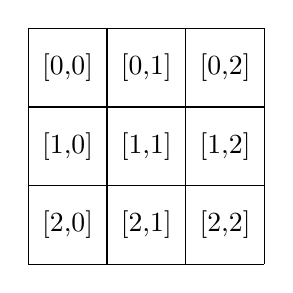
\begin{tikzpicture}
    \draw (0,0) grid (3,3);
    \node at (0.5,2.5) {[0,0]};
    \node at (1.5,2.5) {[0,1]};
    \node at (2.5,2.5) {[0,2]};
    \node at (2.5,1.5) {[1,2]};
    \node at (2.5,0.5) {[2,2]};
    \node at (1.5,0.5) {[2,1]};
    \node at (0.5,0.5) {[2,0]};
    \node at (0.5,1.5) {[1,0]};
    \node at (1.5,1.5) {[1,1]};
  \end{tikzpicture}
  \caption{A small map with annotated locations.}
  \label{table:location}
\end{table}

Though maps appear to be planar, they behave like a torus. Thus, a butterfly
traveling off the east border of a map appears on the west border. Similarly, a
butterfly traveling off the north border of a map appears on the south border.
Figure~\ref{fig:torus} shows a toroidal Earth.

\begin{figure}[h]
    \centering
    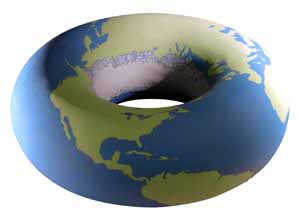
\includegraphics[scale=0.5]{img/torus.jpg}
    \caption{Toroidal Earth. Note that the Earth is not toroidal, and spheres
        cannot be arbitrarily converted to toruses. This is an illustration of
        what the Earth would look like \textit{if it were} a torus.}
    \label{fig:torus}
\end{figure}

\subsubsection{Light}
\removed{}

\subsubsection{Wind}
\removed{}

\subsubsection{Flowers} \label{sec:flowers}
Each tile has zero or more flowers (of class \java{Flower}), which can be
accessed via \java{TileState}'s method \java{getFlowers()}. A flower has a
unique long identifier, \java{flowerId}, and an initial aroma intensity of $1
\times 10^6$, and each flower radiates its aroma about the map\footnote{Really,
a flower will  radiate its aroma only up to \java{Integer.MAX_VALUE} steps
away. We will never test you on maps of such a size, so you can assume that it
radiates its aroma to all \java{Tile}s.}. The aroma at a distance $d$ from a
flower can be calculated as follows.  \[\text{aroma}_d =
\frac{\text{aroma}_{\text{initial}}}{(1 + d)^2}.\] Here, $d$ is the shortest
distance from a tile to a flower. For example, consider the $3 \times 3$ map
with a flower planted in the center as shown in Figure~\ref{table:manhattan} and
Figure~\ref{table:aroma}.  

\begin{table}[H]
  \centering
  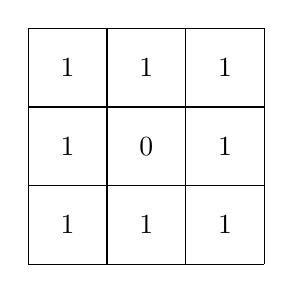
\begin{tikzpicture}
    \draw (0,0) grid (3,3);
    \node at (0.5,2.5) {1};
    \node at (1.5,2.5) {1};
    \node at (2.5,2.5) {1};
    \node at (2.5,1.5) {1};
    \node at (2.5,0.5) {1};
    \node at (1.5,0.5) {1};
    \node at (0.5,0.5) {1};
    \node at (0.5,1.5) {1};
    \node at (1.5,1.5) {0};
  \end{tikzpicture}
  \caption{Distances from the center of the map.}
  \label{table:manhattan}
\end{table}

\begin{table}[H]
  \centering
  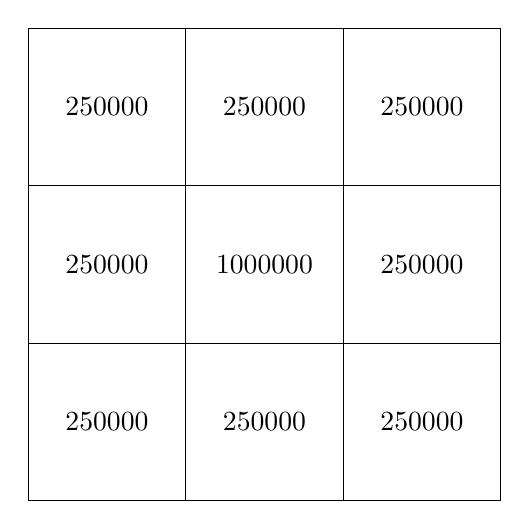
\begin{tikzpicture}
    \draw[step=2cm] (0,0) grid (6,6);
    \node at (1,5) {250000};
    \node at (3,5) {250000};
    \node at (5,5) {250000};
    \node at (5,3) {250000};
    \node at (5,1) {250000};
    \node at (3,1) {250000};
    \node at (1,1) {250000};
    \node at (1,3) {250000};
    \node at (3,3) {1000000};
  \end{tikzpicture}
  \caption{Sample spreading of aroma without obstacles or map wrapping.}
  \label{table:aroma}
\end{table}

Figure~\ref{table:aroma} shows aroma propagation on a simple map without
obstacles or wrapping. However, including these obstacles and wrapping does not
complicate the propagation. The distance $d$ for each tile is still its
shortest distance to the flower. 

\paragraph{Flower Invariants}
\begin{enumerate}
    \item \emph{Each instantiated flower is unique}. Even if two flowers use
      the same image and occupy the same tile, they are distinct. A corollary
      of this invariant is that \emph{no two \java{Flower}s are equal as
      determined by \java{Flower.equals()}}.  
    \item Flowers may bloom (1) before \java{learn} is invoked or (2) after
        \java{learn} terminates and before \java{run} is invoked. \emph{Once a
        flower blooms, it continues to bloom} at the same location for the
        duration of the simulation. Flowers that bloomed in \java{learn} are
        there during \java{run}.
\end{enumerate}

\subsubsection{Aromas}
Each tile has zero or more aromas (of class \java{Aroma}), which can be
accessed using \java{TileState} method \java{getAromas()}. An aroma has an
intensity (in public field \java{intensity}) and an associated \java{flowerId},
a long that will match a \java{Flower} object, once that \java{Flower} is
found.

Each aroma is associated with one specific flower. Aromas of different flowers
are completely independent and are completely separate instantiations of
\java{Aroma}.
\fi

% \ifx \RANDOMMAPCONSTRUCTION \undefined \else
% \subsection{Random Map Construction}\label{sec:mapconstruction}
% If a map file is not provided to Danaus, a randomly generated map is used for
% the simulation. An understanding of the details behind generating a random map
% is not needed\footnote{Though if you are interested, the implementation is in
% Map.java. The algorithms are rather interesting.}, but an understanding of a
% few basic principles is beneficial.
% \begin{itemize}  
%     \item The size of a map is random. There is guaranteed to be at least one
%         \java{Tile}.
%     \item The topology of a map is random\footnote{While the topology of a map
%             is random, it still has some interesting properties. Forests are
%             generally connected and reflect the shape of real world forests
%             ---they tend to be oblong and clustered. Cliffs are generally
%             connected and reflect the shape of real world mountain ranges
%             ---they tend to be long and windy. Land masses on maps, no matter
%             how wide or skinny, tend to scale to the size of the map. Also,
%             fractions of forests, cliffs, and water reflect their real life
%         counterparts on Earth.}.
%     \item A map is guaranteed to be connected: a butterfly can always access
%         all flyable tiles in the map. There will never be \java{Land} or
%         \java{Forest} that cannot be reached.
%     \item Flowers are distributed randomly about the map.
% \end{itemize} 
% \fi
\fi

%%%%%%%%%%%%%%%%%%%%%%%%%%%%%%%%%%%%%%%%%%%%%%%%%%%%%%%%%%%%%%%%%%%%%%%%%%%%%%%%
% BUTTERFLY API
%%%%%%%%%%%%%%%%%%%%%%%%%%%%%%%%%%%%%%%%%%%%%%%%%%%%%%%%%%%%%%%%%%%%%%%%%%%%%%%%
\ifx \BUTTERFLYAPI \undefined \else
\section{Butterfly API}\label{sec:api}
In order to implement your butterfly, you must first create a subclass of
\java{AbstractButterfly}, which defines various public and protected methods
that you use to control your butterfly. For more information on the butterfly
API, refer to the javadoc specifications of the fields and methods.

\ifx \VOIDFLY \undefined \else
\subsection{void fly(Direction heading, Speed s)}
Method \java{fly} attempts to fly your butterfly in \java{Direction heading}
with  \java{Speed s}. A butterfly can attempt to fly to any of its neighboring
tiles using any of the eight cardinal directions.

A flight attempt can fail for several reasons. First, if a butterfly attempts
to fly into a \java{Cliff} or over \java{Water}, an
\java{ObstacleCollisionException} exception is thrown. The \java{Location} of
the \java{Butterfly} is unchanged. 
\fi

\ifx \VOIDFLYSAFE \undefined \else
% \subsection{void flysafe(Direction heading, Speed s)}
% This method behaves exactly like fly, except that an
% \java{ObstacleCollisionException} cannot be thrown. Instead, a large power
% penalty is imposed on the butterfly. This method is intended to be used by
% those with less experience handling exceptions. \emph{It is best not to use
% this method.}
\fi

\ifx \VOIDLAND \undefined \else
\subsection{void land()}
\removed{}
\fi

\ifx \BOOLEANCOLLECT \undefined \else
\subsection{boolean collect(Flower f)}
During the \java{run()} phase, the goal of a butterfly is to collect a set of
flowers. Method \java{collect} attempts to collect \java{Flower f} in the tile
the butterfly is currently on. If \java{f} is planted on the tile, it is
collected and \java{true} is returned; if \java{f}  is not planted on the tile,
\java{false} is returned. 
\fi

\ifx \VOIDREFRESHSTATE \undefined \else
\subsection{void refreshState()}
Every instance of a subclass of \java{AbstractButterfly} has a \java{TileState}
field named \java{state}. When \java{refreshState} is called, \java{state} is
updated with the \java{TileState} of the tile the butterfly is currently on.

Note that if a butterfly flies to a tile, the butterfly's state is \emph{not}
automatically updated. For example, \java{state.location} will contain the
wrong information. It is up to you to call \java{refreshState()} if you want
access to the current tile's \java{TileState}.  
\fi

\ifx \POWERGETPOWER \undefined \else
\subsection{Power getPower()}
\removed{}
\fi

\ifx \INTGETMAPWIDTH \undefined \else
\subsection{int getMapWidth()}
Method \java{getMapWidth} returns the number of columns of the map the
butterfly is on.
\fi

\ifx \INTGETMAPHEIGHT \undefined \else
\subsection{int getMapHeight()}
Method \java{getMapHeight} returns the number of rows of the map the butterfly
is on.
\fi
\fi

%%%%%%%%%%%%%%%%%%%%%%%%%%%%%%%%%%%%%%%%%%%%%%%%%%%%%%%%%%%%%%%%%%%%%%%%%%%%%%%%
% Learning and Running
%%%%%%%%%%%%%%%%%%%%%%%%%%%%%%%%%%%%%%%%%%%%%%%%%%%%%%%%%%%%%%%%%%%%%%%%%%%%%%%%
\ifx \LEARNINGRUNNING \undefined \else
\section{Learning and Running}\label{sec:learnrun}
% Machine learning\footnote{For more information on machine learning, refer to
%     the online resources of Cornell's Introduction to Machine Learning course:
% \link{http://www.cs.cornell.edu/courses/cs4780/2013fa/}{CS 4780}} is a branch
% of artificial intelligence in which a programs can learn from a given set of
% data. Formally, a program is said to learn if its performance as some task
% \emph{T} improves with some experience \emph{E} as measured by some performance
% metric
% \emph{P}\footnote{\link
%     {http://www.cs.cmu.edu/afs/cs.cmu.edu/user/mitchell/ftp/mlbook.html}{Machine
% Learning, Tom Mitchell}}. In danaus, E, T, and P can be described informally as
% follows.
% \begin{itemize}
%     \item \emph{T} Collect an ordered set of flowers on an unfamiliar map.
%     \item \emph{E} Exploring maps populated with flowers.
%     \item \emph{P} Danaus includes a multitude of performance metrics.
% \end{itemize}
% 
% Many machine learning algorithms consists of two phases, which we will refer to
% as learning and running. During learning, the algorithm receives and processes
% sets of training data. This experience is associated with E. During running,
% the algorithm attempts to perform well at task T as measured by P.

Danaus simulations have two phases: learning and running.
\java{AbstractButterfly} declares these phases as two methods:
\java{TileState[][] learn()} and \java{void} \java{run(List<long>}
\java{flowerIds)}. When Danaus is started, it sets up the required
infrastructure to execute a simulation. Once this is complete, it calls your
method \java{learn()}. After some computation and map modifications, it call
method \java{run()}. The details of these two methods and the flow of a
simulation are provided below.

\ifx \LEARNING \undefined \else
\subsection{Learning}
Before \java{learn()} is invoked, Danaus sets up the appropriate framework.
First, it parses arguments to method \java{main}. It decides whether to
instantiate a GUI\@. It randomly generates a map or parses a map from a map
file.  It instantiates an instance of your butterfly and places it on the map.
It invokes your implementation of \java{learn()}. 

The purpose of \java{learn()} is for a butterfly to explore and save the
flyable tiles of a map. It does so by generating and returning a
two-dimensional array of \java{TileState}s, whose flyable tiles must match the
map's \java{TileState}s. Danaus then determines how well the map and the
returned array match. \java{TileState}s do not have to be provided for
\java{Cliff} or \java{Water} tiles. Any \java{TileState}, or null, can be
provided and will be counted as a correct.

During the learning phase of a simulation, you \emph{should not and cannot}
collect flowers. An attempt to collect a flower during \java{learn()} will
throw a \java{PrematureCollectionException}, and no flower will be collected.

Instead, focus on collecting the required information about the map as
efficiently as possible. You are required to return a two-dimensional array of
\java{TileState}s that contains the information in all flyable states of the
map. It is up to you to determine how to explore the map to do this. 
\fi

\ifx \RUNNING \undefined \else
\subsection{Running}
After the \java{learn()} phase, Danaus shifts to the running phase of the
simulation. First, Danaus  randomly adds more flowers to the map and spreads
their aromas. (Other than the new flowers and aromas, the map does not change.
The location of the butterfly and all the information it has saved up to this
point is also maintained.)

Next, Danaus  randomly generates a list of flower id's and passes this list to
your method \java{run()}. The list may contain some flower id's belonging to
flowers that were initially on the map as well as flowers that were added after
\java{learn()} terminated. The goal is to collect the associated flowers as
efficiently as possible --- \emph{the order in which they are collected does
not matter.}

Before having the butterfly fly around and collect flowers, your method
\java{run()} should use the two-dimensional \java{TileState} array that was
constructed during the \java{learn()} phase to figure out how to fly around and
collect flowers as efficiently as possible. There are many ways to do this.
Coding a correct, readable, well-documented, and efficient butterfly during the
\java{run} phase is the core challenge and fun of Danaus.

Once \java{run} terminates, Danaus checks the collected flowers against the
list of flowers given to \java{run}. If your butterfly collected every flower
\emph{(and only those) in any order}, you successfully complete the simulation.
\fi
\fi

%%%%%%%%%%%%%%%%%%%%%%%%%%%%%%%%%%%%%%%%%%%%%%%%%%%%%%%%%%%%%%%%%%%%%%%%%%%%%%%%
% Command Line Options
%%%%%%%%%%%%%%%%%%%%%%%%%%%%%%%%%%%%%%%%%%%%%%%%%%%%%%%%%%%%%%%%%%%%%%%%%%%%%%%%
\ifx \CLO \undefined \else
\section{Command Line Options}
Danaus has various command-line options that affect execution of a simulation,
and you may want to alter the execution by providing some of them. Most
students will be running using Eclipse, and we now explain how to give
command-line arguments in Eclipse.

With the Danaus project selected in the Package Explorer, click \emph{``Run''}
at the top of the screen. Then, click \emph{``Run Configurations''}. A windowed
menu pops up. You  see a tab titled \emph{``Arguments''} near the top of the
screen next to the \emph{``Main''} and \emph{``JRE''} tabs. Click on the
\emph{``Arguments''} tab. The topmost text box is titled \emph{``Program
arguments:''}. This is where you enter your command line options.

Here is a list of the options Danaus provides. Arguments can appear in any
order. Text in bold should be entered literally. While italicized text should
be replaced with the appropriate arguments.
\begin{itemize}
    \item \emph{\java{--help}}\\
        Print a friendly help message and exit the program. 

    \item \emph{\java{-h, --headless}}\\
        Run Danaus without a GUI.

    \item \emph{\java{-d, --debug}}\\
        Danaus keeps track of various debugging information. When this option
        is provided, the debugging information is printed to the screen.

    \item \emph{\java{-w, --warning}}\\
        Danaus keeps track of various warning information. When this option is
        provided, the warning information is printed to the screen.

    \item \emph{\java{-i, --infinite}}\\
        \removed{}

    \item \emph{\java{-s, --seed <seed>}}\\
        Danaus uses a single psuedo-random number generator to generate its
        randomness. A psuedo-random number generator creates a string of
        apparently random numbers from an initial seed. If you specify a seed,
        Danaus repeatedly produces the ``random'' map generated from that seed. 

    \item \emph{\java{-f, --file <mapfile>}}\\
        If a map file is provided, Danaus generates the map from the map file
        instead of randomly generating the map.
\end{itemize}

In addition to these command-line options, you can also provide command-line
arguments.
Unlike options, arguments do not require a ``\java{-}'' or ``\java{--}''.

The only command line arguments Danaus accepts are the names of the butterfly
classes you want to run the simulation with. For example, if
\java{CornellButterfly} is a subclass of \java{AbstractButterfly}, you can run
Danaus as follows:
\begin{Java}
  java danaus.Simulator student.CornellButterfly
\end{Java}
Or, if  running Danaus from Eclipse, simply put ``\java{CornellButterfly}'' in
the \emph{``Program arguments:''} tab, as described above. If several class
names are provided, the first class is used. If no class names are provided,
the name ``\java{Butterfly}'' is used by default.

For more information on Danaus' command line options, refer to Danaus' man page
located in \java{/doc/man}. For more information on man pages or if you are
having trouble using the Danaus command-line options, refer to Google, Piazza,
or ask a professor, TA, consultant, or friend.
\fi

%%%%%%%%%%%%%%%%%%%%%%%%%%%%%%%%%%%%%%%%%%%%%%%%%%%%%%%%%%%%%%%%%%%%%%%%%%%%%%%%
% Some Advice From Me To You
%%%%%%%%%%%%%%%%%%%%%%%%%%%%%%%%%%%%%%%%%%%%%%%%%%%%%%%%%%%%%%%%%%%%%%%%%%%%%%%%
\ifx \ADVICE \undefined \else
% \section{Some Advice From Me To You}
% Danaus can seem like a large and insurmountable challenge at first, especially
% for students learning how to program. A maelstrom of graph exploration, Danaus
% can be an intimidating beast. However, Danaus isn't as scary as it seems.
% Retrospectively, you will likely find the experience easy and fun. Here is some
% advice to help alleviate stress and ensure you learn a lot, have fun, and get a
% good grade.
% \begin{itemize}
%     \item \emph{Start early!} If you're a particularly adept programmer, you
%         may be tempted to complete Danaus' assignments the night before they
%         are due. This won't work.
%     \item \emph{Read, read, read.} Your implementation may be beautiful and
%         efficient, but if it doesn't do what is required, you have little
%         chance of success. Make sure you read through what we expect you to do
%         and how we expect you to do it.
%     \item \emph{Plan.} Architects don't build buildings until they've drawn
%         blueprints. Computer scientists should be no different. Think about
%         your algorithms before you write them. Talk them over with your
%         partner, if you have one.
%     \item \emph{Get help.} If you've read this document early and planned
%         things out but are still confused, ask someone for help. You may have a
%         friend that has a better understanding of what to do. If not, ask a
%         consultant, TA, or professor. Go to their office hours or send them an
%         email. You have an army of staff ready, willing, and eager to help you
%         out.
%     \item \emph{Adjust to your comfort.} If you are uneasy about your
%         programming skills, write a simple solution. If you are more
%         comfortable with programming, write an efficient solution. If you are
%         an ``1337 h4x0r'', then optimize your code until  the cows come home.
%         No matter what level of expertise you are, adjust Danaus to meet your
%         needs. You can get a good grade on the assignment no matter how adept
%         you are.  
%     \item \emph{Have fun and learn a lot!} CS 2110 is the foundation for your
%         career as a computer scientist. Enjoy it and learn from it! 
% \end{itemize}
\fi

%%%%%%%%%%%%%%%%%%%%%%%%%%%%%%%%%%%%%%%%%%%%%%%%%%%%%%%%%%%%%%%%%%%%%%%%%%%%%%%%
% Credits
%%%%%%%%%%%%%%%%%%%%%%%%%%%%%%%%%%%%%%%%%%%%%%%%%%%%%%%%%%%%%%%%%%%%%%%%%%%%%%%%
\ifx \CREDITS \undefined \else
\section{Credits}
Many thanks to all those who contributed to the creation of Danaus and allowed
us to use their work. Without them, Danaus would not be as complete or as
elegant as it is with their contributions.

\begin{itemize}
    \item Flower sprites were taken from
        \link
        {http://neoriceisgood.deviantart.com/art/100-Flower-Sprites-348880673}
        {neorice}.
    \item Butterfly sprites were taken from
        \link{http://toadstone.tumblr.com/}{David Nyari}. 
\end{itemize}
\fi

\end{document}
